\documentclass[letterpaper,11pt]{book}
\usepackage{bm}
\usepackage{graphicx}
\usepackage{amsmath}
\usepackage{amssymb}
\usepackage{mathrsfs}
\usepackage{bbold}
\usepackage{braket}
\usepackage{color}
\usepackage{subfigure}
\usepackage{hyperref}

\begin{document}

\chapter{Phase Coherence}
\section{Off-Diagonal Long Range Order}
Bose Einstein condensation, off diagonal long range order, and phase coherence are three concepts which connect to each other. The relation among them became clearer in the recent years.
The concept of Bose Einstein condensation origins from Liquid Helium i.e.  superfluid $^4He$, superconductor $^3He$ and so on. Later on, the concept of supersolid came out. 
They are all popular questions during 1940s or 1950s. The questions are how to understand $He$. All of these are called Macroscopic Quantum Phenomena. 
When we mention Superfluid, it means a brunch of things in phenomenology. All the phenomena come from the Broken Gauge Symmetry. 

Firstly, the broken gauge symmetry automatically implies the superfluid velocity. The superfluid velocity describes the motion, also related to super-current, leading to the quantization of circulations. All of them refer to the phenomenon that if there is a current going around a closed loop, the current will last for long time, in the sense of "forever" in principle. This phenomenon never happens in water. See Figure \ref{fig:1-1}.

\begin{figure}[htbp]
\centering
%\includegraphics[width=4in]{image/} 
\caption{Super-Current}
\label{fig:1-1}
\end{figure}


Secondly, if we rotate the liquid, we could observe the lattice of vortexes, which never happens in normal fluid such as flashing a toilet. See Figure \ref{fig:1-2}.

\begin{figure}[htbp]
\centering
%\includegraphics[width=4in]{image/} 
\caption{Vortex Lattice}
\label{fig:1-2}
\end{figure}


There is a two-fluid picture due to Landau. Landau said the fluid contains two parts, one of which has zero entropy referring to the "condensate" nowadays. The picture has a great insight. Based on this picture, we could picture this kind of fluid, due to experiments, in to the following equation:
\begin{equation}
\text{Hellium} = \text{Part with zero entropy} + \text{Part of excitations carring entropy}.
\end{equation}
One of the most famous experiments is called "Fountain Effect". See Figure \ref{fig:1-3}.

\begin{figure}[htbp]
\centering
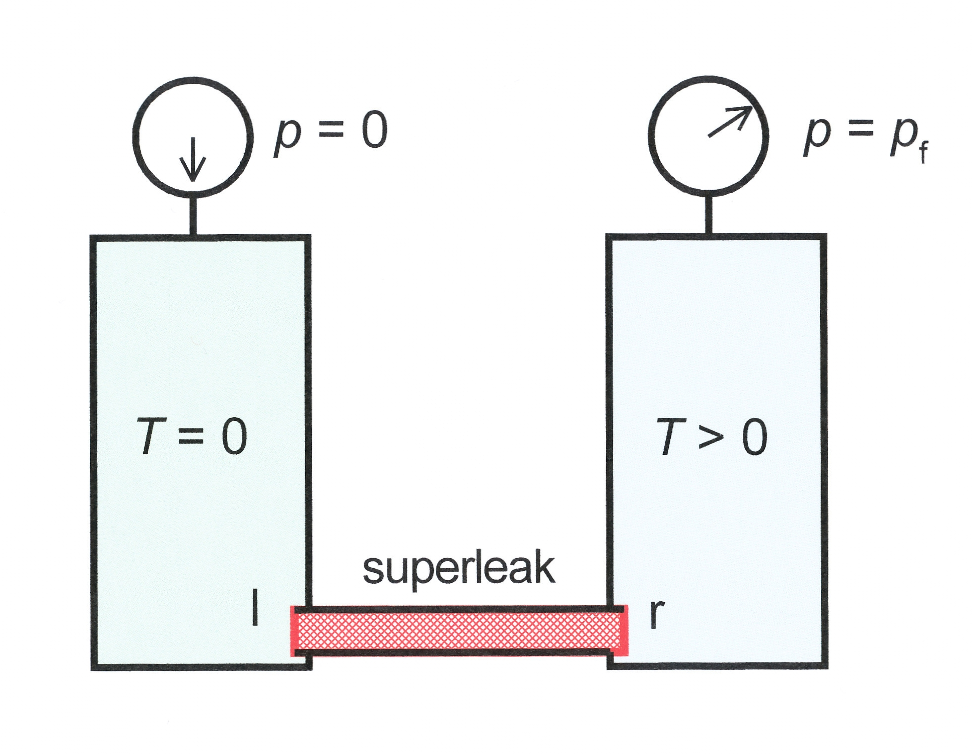
\includegraphics[width=4in]{image/1-3-fountain.pdf} 
\caption{Fountain Effect}
\label{fig:1-3}
\end{figure}

Two containers A and B are connected by a very narrow tube. Initially, two containers are both filled by liquid Helium, with the same height and temperature. Then we increase the pressure in container B. As a result, the liquid in B could flow to A. We could observe that the height in A is higher than B and the temperature in B becomes higher than A.

This experiment could be understood by the two-fluid picture. The component passing through the tube carries zero entropy. During the experiment, the volume of the liquid in B decreases and the total entropy preserves; therefore, the entropy density increases. As a result, temperature increases.

So this is the general picture. And Landau PROPOSED that the component with zero entropy could be described by a BIG WAVEFUNCTION $\Psi(\bm r)$. If taking a look at his original paper, you would not know where it comes from. It is just a proposal. Landau somehow felt that in the system there is such a thing, i.e. a macroscopic wave function. 

A significant property is that the macroscopic wave function is complex, which has a phase $\Psi(\bm r)= |\Psi(\bm r)|e^{i\theta}$. And the phase will lead to all the phenomena we mentioned above.

This is Landau's picture. Based on this, Landau created and derived the two-fluid superfluid dynamics theory. The superfluid dynamics theory contains a sequence of equations, which has been tested by experiments extremely well.

In those days, it seems that in fact there is such a thing, i.e. a macroscopic wavefunction. And later on, Landau proposed the similar thing in superconductivity, which is so called Ginzburg-Landau theory. 

So, here comes the question: what is the "zero entropy component"? 
London first questioned that whether the phenomena in Helium is a sign of Bose Einstein Condensation. However, the original discussion of BEC is for non-interacting systems, while Helium is strongly interacting. So the first step is how could we generalize the concept of BEC to interacting systems.

It turns out that there is a brilliant solution given by Penrose and Onsager. It is called Penrose-Onsager characterization. And it becomes the current way to describe BEC. It actually is not clear how they came to that idea. And I suppose it should have relation to the Landau's Helium theory.  

They consider the density matrix. 
\begin{equation}
\rho(\bm r, \bm r') = \braket{\psi^\dag(\bm r')\psi(\bm r)}
\end{equation}
Penrose and Onsager point out that BEC do have a generalization if we take a look at the density matrix.
It is called matrix as we could treat it in a discrete space, saying $\bm r$ and $\bm r'$ as $i$ and $j$. It is easy to test that the density matrix is a Hermitian matrix, i.e. $\rho(\bm r, \bm r') = \rho(\bm r, \bm r')^\dag$. 

For an arbitrary Hermitian matrix $M=M^\dag$, it should have a spectrum composition.
\begin{equation}
M=\sum_n \lambda_n \ket{n}\bra{n}
\end{equation}
and 
\begin{equation}
M_{ij} = \sum_n \lambda_n \braket{i|n}\braket{n|j}
\end{equation}
Here $\lambda$ should be real. 

So the density matrix could be written in a general form
\begin{equation} 
\rho(\bm r, \bm r') = \sum_n \lambda_n v_n^\star(\bm r') v_n(\bm r)
\end{equation}
where $\lambda_n$ is the eigenvalue and $v_n(\bm r)$ is normalized.
\begin{equation}
\int d \bm r |v_n(\bm r)|^2 = 1 
\end{equation}

It is not hard to show that the eigenvalue $\lambda_n$ is not only real, but also positive.
The proposal is the following. If we have all the eigenvalues. We could sort the eigenvalues decently, i.e. $\lambda_i \geq \lambda_{i+1}$.   
It is still the general structure of density matrix. 
BEC means the following: there is only one big eigenvalue, while others are very weak. More mathematically, (See Figure \ref{fig:1-4})
\begin{eqnarray}
\lambda_0 &\sim & \mathscr{O}(N)\\
\lim_{N\rightarrow \infty}\frac{\lambda_n}{\lambda_0} &\rightarrow & 0
\end{eqnarray}

\begin{figure}[htbp]
\centering
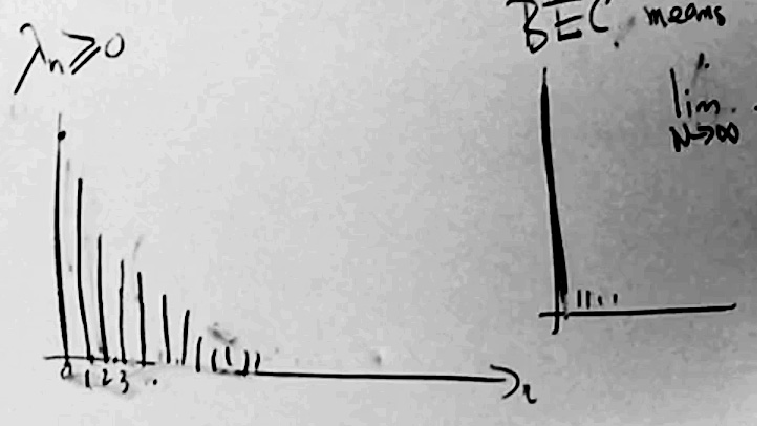
\includegraphics[width=4in]{image/1-4-bec.pdf} 
\caption{BEC and eigenvalues of density matrix.}
\label{fig:1-4}
\end{figure}

BEC is one special situation: only one of the eigenvalues are big and the others are small. We say it is small, in the sense of the comparison with the big eigenvalue. For example, in the solid materials, $N$ is about $10^{23}$. And the sum of all the other eigenvalues could be around $10^10$, then the ratio should be treated as zero, i.e. very small eigenvalues. However, the exact number is still very huge, i.e. $10^{10}$. 

Currently, we only give the DEFINITION. The question is whether it is a useful concept and how general it is. It is refer to the fragmented condensate. 

Comments: What if we have two big eigenvalues? Or even more eigenvalues? All of them are in the same order (not need to be equal) and the rest of them are small. They are more unusual situations. It is hard to see and several general arguments are for them. They could and could not be related to the degenerate ground states. The degenerate ground states is one of the probabilities.

In the following we discrete the variables to make it clear 
\begin{eqnarray}
\rho(r,r') &=& \lambda_0 v_0^\star(r')v_0(r) \\
&=& \lambda_0 \left(\begin{array}{c}
v^\star(r_1)\\
v^\star(r_2)\\
\cdots\\
v^\star(r_m)\\
\end{array}\right) 
\left(\begin{array}{cccc} v(r_1)& v(r_2)&\cdots & v(r_m)\\ \end{array}\right)\\
&=& \lambda_0 
\left(\begin{array}{cccc}
v^\star(r_1)v(r_1)& v^\star(r_1)v(r_2)&\cdots & v^\star(r_1)v(r_m)\\
v^\star(r_2)v(r_1)& v^\star(r_2)v(r_2)&\cdots & v^\star(r_2)v(r_m)\\
\cdots& \cdots&\cdots & \cdots\\
v^\star(r_m)v(r_1)& v^\star(r_m)v(r_2)&\cdots & v^\star(r_m)v(r_m)\\
\end{array}\right)
\end{eqnarray}

The density matrix got non-zero elements everywhere, not only along the diagonal. It could be non-zero far away from the diagonal, even at the corner of the matrix, $v^\star(r_1)v(r_m)$. Therefore, it comes to the concept, Off-Diagonal Long Range Order(ODLRO). It means the corner element is still huge in the order of $\lambda_0$, the maximum eigenvalue. 

As $v_0$ is complex, all the matrix elements in $\rho(r,r')$ is complex, carrying a phase, which refers to the concept of phase coherence. 

More definitions,
\begin{equation}
\Psi_0(r) = \sqrt{\lambda_0} v_0(r)
\end{equation}
Then 
\begin{equation}
\int dr |\Psi_0(r)|^2 = \lambda_0
\end{equation}
This is the condensate wavefunction. It is the macroscopic wavefunction in Landau's theory. 

Example 1: Free Particle System.
\begin{eqnarray}
\braket{\psi^\dag(\bm r')\psi(\bm r)} &=& \sum_k \frac{e^{i \bm k \cdot (\bm r-\bm r')}}{V}n_k(T)\\
&=& \left\{\begin{array}{cc}
n_0(T) + \int \frac{d \bm k}{8\pi^3} \frac{e^{i \bm k \cdot (\bm r-\bm r')}}{e^{k^2/2mT}-1} & T < T_c\\
\int \frac{d \bm k}{8\pi^3} \frac{e^{i \bm k \cdot (\bm r-\bm r')}}{e^{(k^2/2m+|\mu|)/T}-1} & T > T_c\\
\end{array}\right. 
\end{eqnarray}
\textit{Comments: chemical potential $\mu$ in the free Bose gas.
When $T>T_c$, $\mu < 0$. When $T<T_c$ starting to condense, $\mu = 0$.}

We could show that the integral in the above approaches $0$ when $|\bm r-\bm r'|\rightarrow \infty$. 
Therefore, at high temperature $T>T_c$, there is no off-diagonal long range order. And the eigenvalue of the density matrix are 
\begin{equation}
n(k) = \frac{1}{e^{(k^2/2m+|\mu|)/T}-1} 
\end{equation}
When $T<T_c$, there is something coming out at $k=0$, say $n_0(T)$.
And eventually at very low temperature, all $n(k)$ become very small and $n_0(T)$ becomes very large to the order of $N$. 
When $T\rightarrow 0$, the integral gives us $0$, and all the elements in the density matrix become $n_0(T=0)$ even far away from the diagonal.
See figure \ref{fig:1-5}.

\begin{figure}[htbp]
\centering
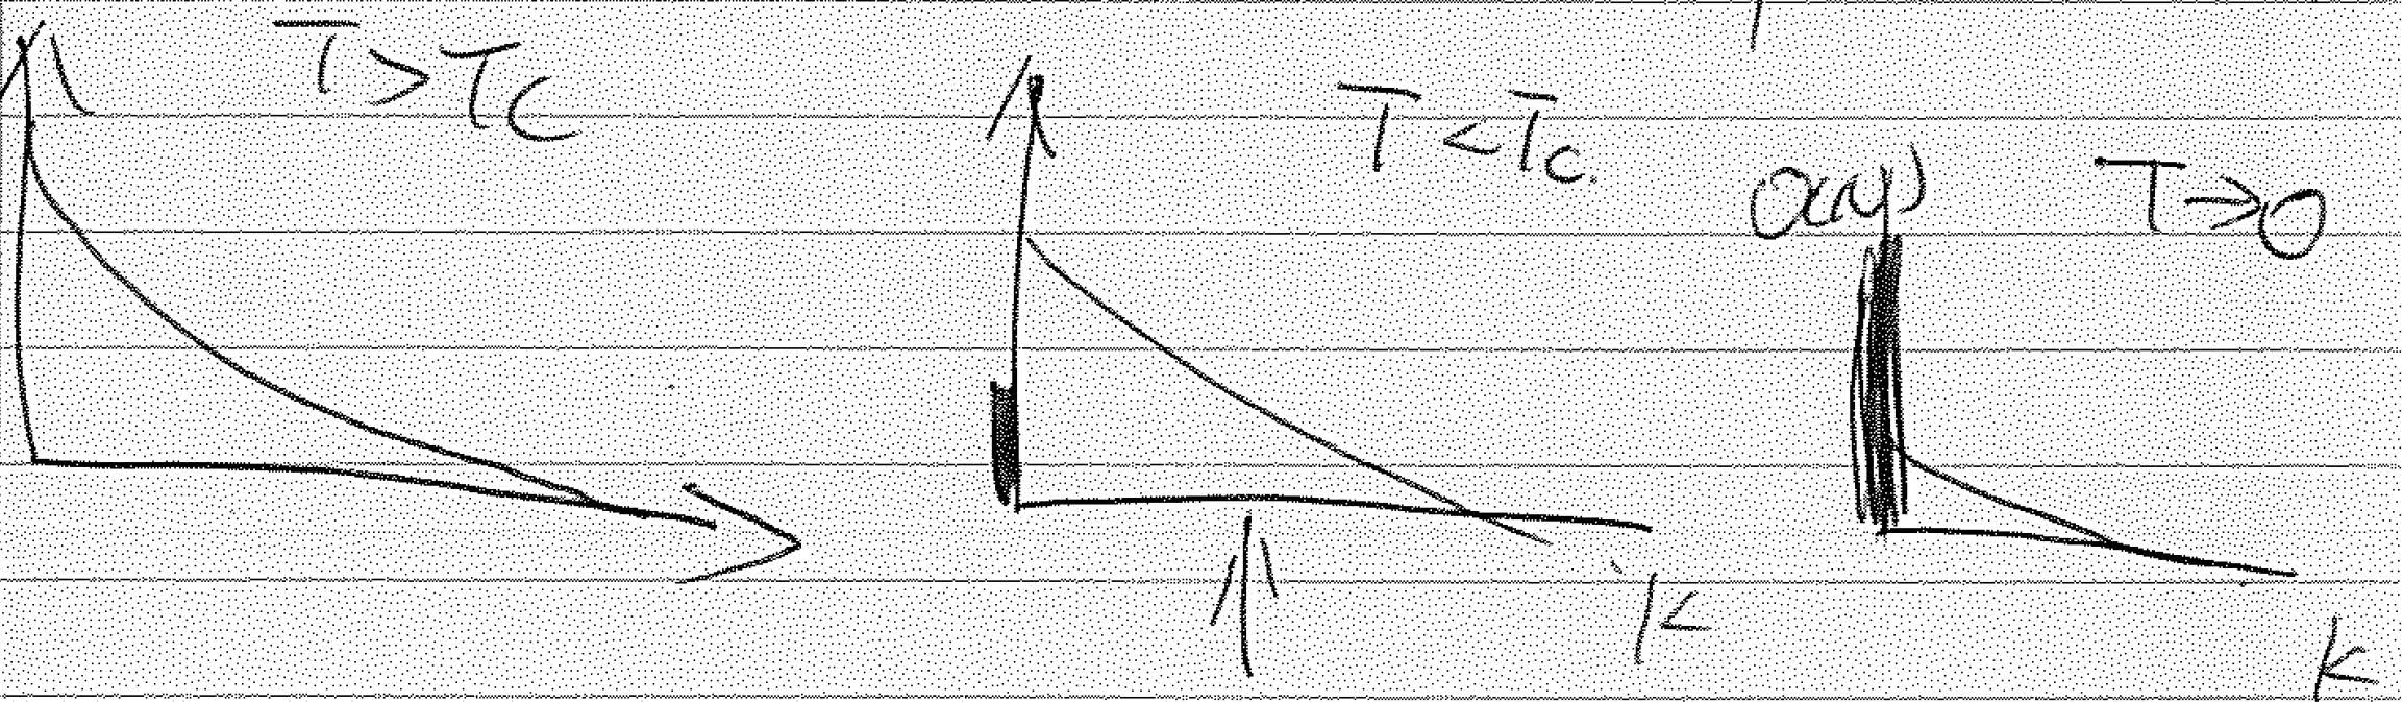
\includegraphics[width=4in]{image/1-5-free_bose.pdf} 
\caption{Free Bose Gas}
\label{fig:1-5}
\end{figure}

Example 2: Consider the following state
\begin{equation}
\ket{\Psi} = \frac{1}{\sqrt{N!}}\left(\int d\bm r \nu(\bm r) \psi^\dag(\bm r)\right)^N\ket{vac}
\end{equation}
where $\nu(\bm r)$ is normalized wavefunction, i.e.
\begin{equation}
\int d\bm r |\nu(\bm r)|^2 = 1
\end{equation}
and $\psi^\dag(\bm r)$ is the Bosonic creation operator.
We could check
\begin{equation}
\braket{\psi^\dag(\bm r') \psi(\bm r)} = N \nu^*(\bm r')\nu(\bm r)
\end{equation}
\footnote{We could check the equation easily
\begin{eqnarray}
\psi(\bm r) \ket{\Psi} &=& \frac{1}{\sqrt{N!}} \psi(\bm r)\left(\int d\bm x \nu(\bm x) \psi^\dag(\bm x)\right)^N\ket{vac}\notag\\
&=& \frac{1}{\sqrt{N!}} \left\{N \nu(\bm r) \left(\int d\bm x \nu(\bm x) \psi^\dag(\bm x)\right)^{N-1}+\left(\int d\bm x \nu(\bm x) \psi^\dag(\bm x)\right)^N\psi(\bm r)\right\} \ket{vac}\notag\\
&=&\frac{1}{\sqrt{N!}}N \nu(\bm r) \left(\int d\bm x \nu(\bm x) \psi^\dag(\bm x)\right)^{N-1} \ket{vac}\notag
\end{eqnarray}
Then
\begin{eqnarray}
\braket{\Psi|\psi^\dag(\bm r') \psi(\bm r)|\Psi} &=& \frac{1}{N!} N^2 \nu^*(\bm r')\nu(\bm r)\braket{vac|\left(\int d\bm x \nu^*(\bm x) \psi(\bm x)\right)^{N-1} \left(\int d\bm x \nu(\bm x) \psi^\dag(\bm x)\right)^{N-1} |vac}\notag\\
&=& N \nu^*(\bm r')\nu(\bm r)\notag
\end{eqnarray}
}

This relation shows that this system is full condensate. 

Example 3: Penrose \& Onsager's demonstration of ODLRO (BEC)
Considering interacting Bose gas, P\& O proposed a variational wavefunction for the ground state.
\begin{equation}
\Psi(\bm r_1,\ldots,\bm r_N) =\mathscr C \prod_{i>j} f(\bm r_i-\bm r_j)
\end{equation}
where $\mathscr C$ is the normalized constant and $f(\bm r)$ is a real function changing dramatically around $r = \sigma$. A sketch is shown in Fig \ref{fig:1-6}.
It means that due to the interaction, Bosons would like to leave away from each other. If it is hard core, $f(0) = 0$. Outside a certain region, the Bosons don't influence with each other, i,e, $f(r>\sigma) = 1$
We could define $V(\bm r)$ as 
\begin{equation}
f(\bm r) = e^{-V(\bm r)/2 T}
\end{equation}
where $T$ is a positive parameter with the dimension of energy. 
And $f(\bm r)$ satisfies the following approximation perfect
\begin{equation}
f^2(\bm r) \approx f(\bm r)
\end{equation}



\begin{figure}[htbp]
\centering
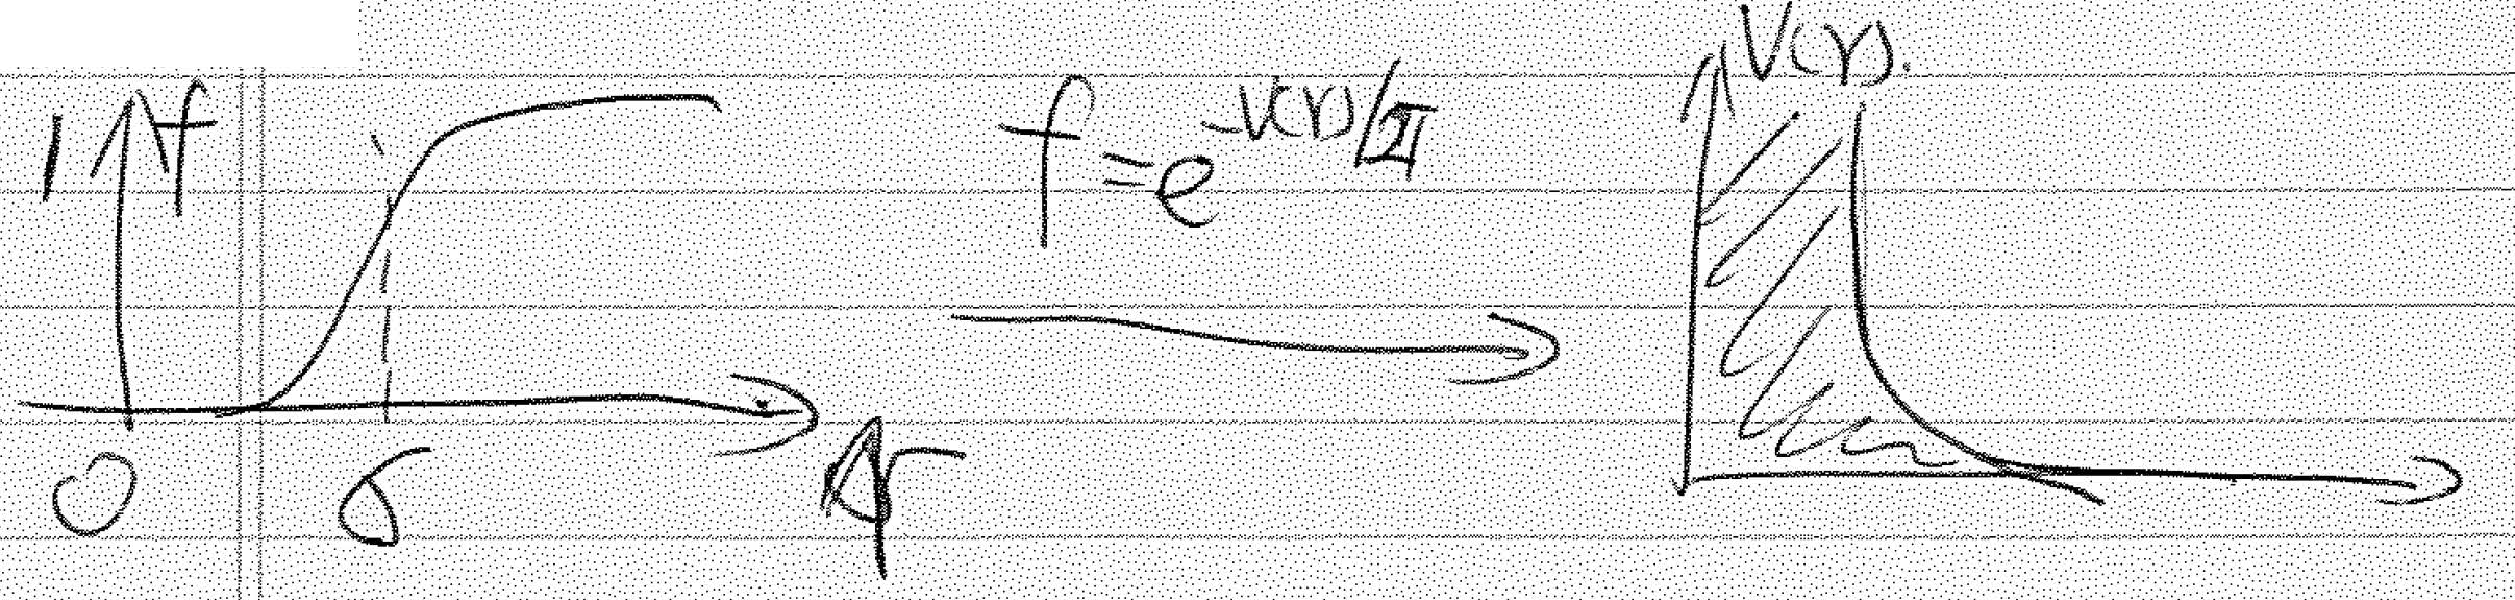
\includegraphics[width=4in]{image/1-6-var_func.pdf} 
\caption{variational wavefunction}
\label{fig:1-6}
\end{figure}

Thus the wavefunction
\begin{equation}
\Psi(\bm r_1,\ldots,\bm r_N) =\mathscr C e^{-\sum_{i>j}V(\bm r_i-\bm r_j)/2T}
\end{equation}

Then 
\begin{eqnarray}
\braket{\psi^\dag(\bm r')\psi(\bm r)} &=& N \int \prod_{i=2}^N d\bm r_i \Psi^*(\bm r',\ldots,\bm r_N)\Psi(\bm r,\ldots,\bm r_N)\notag\\
&=& N \mathscr C^2\int \prod_{i=2}^N d\bm r_i e^{-\sum_{j=2}^N (V(\bm r-\bm r_j)+V(\bm r'-\bm r_j))/2T} e^{-\sum_{i>j|_2^N} V(\bm r_i-\bm r_j)/T}\notag\\
&\approx& N \mathscr C^2\int \prod_{i=2}^N d\bm r_i e^{-\sum_{j=2}^N (V(\bm r-\bm r_j)+V(\bm r'-\bm r_j))/T} e^{-\sum_{1\leq j<i\leq N} V(\bm r_i-\bm r_j)/T}\notag\\
\end{eqnarray}

On the other hand, consider a classical system with $N+1$ particles. The density-density correlation is 
\begin{equation}
\braket{n(\bm r)n(\bm r')}^{(N+1)}_{CL} = \frac{\int \prod_{i=1}^{N+1} d\bm r_i\sum_{i,j} \delta(\bm r-\bm r_i)\delta(\bm r'-\bm r_j) e^{-\sum_{1\leq j<i\leq N+1}V(\bm r_i-\bm r_j)/T}}{Z^{(N+1)}_{CL}}
\end{equation}
where the partition function
\begin{equation}
Z^{(N+1)}_{CL} = \int \prod_{i=1}^{N+1} d\bm r_i \sum_{i,j} e^{-\sum_{1\leq j<i\leq N+1}V(\bm r_i-\bm r_j)/T}
\end{equation}

More concretely
\begin{equation}
\braket{n(\bm r)n(\bm r')}^{(N+1)}_{CL} = \frac{N(N+1)}{2Z^{(N+1)}_{CL}} \int \prod_{i=2}^N d\bm r_i e^{-\sum_{j=2}^N (V(\bm r-\bm r_j)+V(\bm r'-\bm r_j))/T} e^{-\sum_{1\leq j<i\leq N} V(\bm r_i-\bm r_j)/T} 
\end{equation}

Thus 
\begin{equation}
\braket{\psi^\dag(\bm r')\psi(\bm r)} \propto \braket{n(\bm r)n(\bm r')}^{(N+1)}_{CL}
\end{equation}

The proportional ration depends on $N$ surely, but it is independent of $\bm r$ and $\bm r'$.
However,for the classical system with uniform potential under the short-range interaction (for example, classical fluid), we have $\braket{n(\bm r)n(\bm r')} = \bar n_0^2$ under the long range limit, i.e. $|\bm r-\bm r'| \rightarrow \infty$
Thus $\braket{\psi^\dag(\bm r')\psi(\bm r)}$ is finite under the long range limit, i.e. ODLRO. 

Thus we could conclude that the variational wavefunction proposed by P \& O has ODLRO, although it is very complicated, even we don't know the exact form. 


\section{Destroy of Phase Coherence through Interaction}

Consider 2-site Boson Hubbard Model with fixed particle number $N$.
The Hamiltonian is given by
\begin{equation}
H = -t a_1^\dag a_2 -t a_2^\dag a_1 +\frac{U}{2} n_1(n_1-1) +\frac{U}{2} n_2(n_2-1)
\end{equation}
where $a_{i}^\dag (a_{i})$ is the creation (annihilation) operator on site $i (i=1, 2)$, and $n_{1(2)} = a^\dag_{1(2)}a_{1(2)}$ is the particle number on site $1(2)$. $t$ is the hopping amplitude between site 1 and site 2, and $U$ is the on-site interaction strength.
This model could describe the double-well Boson system and bilayer Boson system, shown in Figure \ref{fig:1-7}. 


\begin{figure}[htbp]
\centering
\subfigure[Double Well Boson System]
{
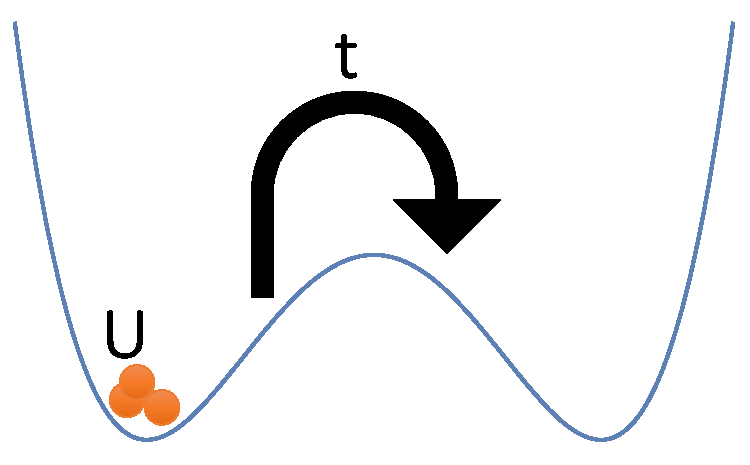
\includegraphics[width=2in]{image/1-7-a2well.pdf}
}
\subfigure[Bilayer Boson System]
{
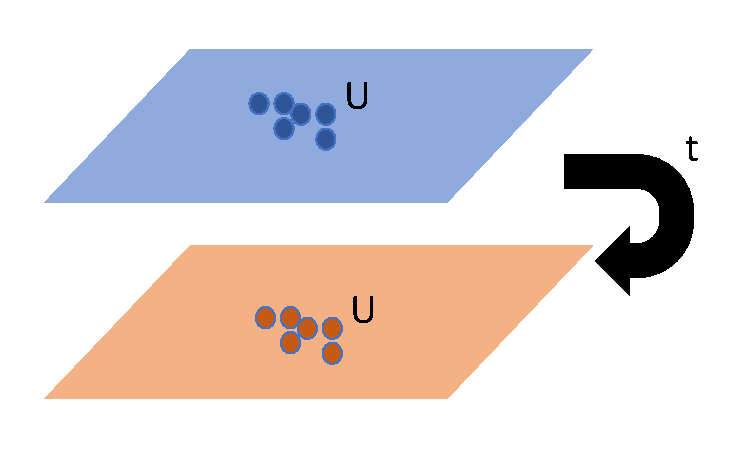
\includegraphics[width=2in]{image/1-7-b2layer.pdf}
}
\caption{Physical system to realize 2-site Bose Hubbard Model}
\label{fig:1-7}
\end{figure}

The total number of particle $N = n_1 + n_2$ is a constant.
Then the Hamiltonian could be written in the form
\begin{equation}
H = -t a_1^\dag a_2 -t a_2^\dag a_1+\frac{U}{4}(n_1-n_2)^2+\frac{U}{4}N(N-2)
\end{equation}
The last term $\frac{U}{4}N(N-2)$ is a constant which only contribute an energy shift in the energy spectrum. As a result, it could be ignored in the following.

\subsection{Three Limits of Interaction}
Instead of consider an arbitrary interaction, firstly we shall focus on three limits of interaction in the following, i.e.
\begin{enumerate}
\item $U=0$
\item $U=+\infty$
\item $U=-\infty$
\end{enumerate}

\subsubsection{Non-interaction $U = 0$}

The ground state is given by
\begin{equation}
\ket{U=0} = \frac{1}{\sqrt{N!}}\left(\frac{a_1^\dag+a_2^\dag}{\sqrt{2}}\right)^N \ket{vac}
\end{equation}
The state is called Coherent State, as all the Bosons are in the same state. The single-particle density matrix
\begin{equation}
\rho=\braket{a_i^\dag a_j} = N\left(\begin{array}{cc}
1/2 & 1/2\\
1/2 & 1/2
\end{array}\right)
\end{equation}
Here we apply the relation
\begin{equation}
a_{1(2)} \left(\frac{a_1^\dag+a_2^\dag}{\sqrt{2}}\right)^N = \frac{N}{\sqrt{2}}\left(\frac{a_1^\dag+a_2^\dag}{\sqrt{2}}\right)^{N-1}+\left(\frac{a_1^\dag+a_2^\dag}{\sqrt{2}}\right)^N a_{1(2)}
\end{equation}
We could have
\begin{eqnarray}
\braket{n_1} &=& N/2\\
\braket{n_1^2} &=& N(N+1)/4
\end{eqnarray}
The fluctuation of particle number on a single site, 
\begin{equation}
\Delta n_1 = \sqrt{\braket{n_1^2}-\braket{n_1}^2} = \sqrt{N}/2
\end{equation}
Then
\begin{equation}
\frac{\Delta n_1}{n_1} = \frac{1}{\sqrt{N}} \rightarrow 0 (N\rightarrow +\infty)
\end{equation}

\subsubsection{Infinite Repulsive Interaction $U=+\infty$}

The ground state is given by
\begin{equation}
\ket{U = +\infty} = \frac{1}{(N/2)!}a_1^{\dag N/2}a_2^{\dag N/2}\ket{vac}
\end{equation}
It is called Fock State. Half of the particles are on site 1, the others are on the other site. The single particle density matrix
\begin{equation}
\rho=\braket{a_i^\dag a_j} = N\left(\begin{array}{cc}
1/2 & 0\\
0 & 1/2
\end{array}\right)
\end{equation}
Then
\begin{eqnarray}
\braket{n_1} &=& N/2\\
\braket{n_1^2} &=& N^2/4
\end{eqnarray}
The fluctuation of particle number on a single site,
\begin{equation}
\Delta n_1 = 0
\end{equation}

\subsubsection{Infinite Attractive Interaction $U=-\infty$}

Without hopping term, the ground state is doubly degenerate, $a_1^{\dag N}$ and $a_2^{\dag N}$.
The finite hopping could couple the degenerate ground states, and the even in $N$-th order. And the even parity state gives the lowest energy.
\begin{equation}
\ket{U = -\infty} = \frac{1}{\sqrt{2}\sqrt{N!}}\left(a_1^{\dag N} + a_2^{\dag N}\right)\ket{vac}
\end{equation}
It is called Schrodinger's Cat State. The system is in a superposed state.

The single particle density matrix
\begin{equation}
\rho=\braket{a_i^\dag a_j} = N\left(\begin{array}{cc}
1/2 & 0\\
0 & 1/2
\end{array}\right)
\end{equation}
Then
\begin{eqnarray}
\braket{n_1} &=& N/2\\
\braket{n_1^2} &=& N^2/2
\end{eqnarray}
The fluctuation of particle number on a single site,
\begin{equation}
\Delta n_1 = N/2
\end{equation}
Then
\begin{equation}
\frac{\Delta n_1}{n_1} = 1
\end{equation}
\subsubsection{A brief summary of the three limit cases}
A brief summary of the three limit cases are shown in Table \ref{tab:1-1-2BoseLmt}.
\begin{table}[htbp]
\centering
\caption{2-site Bose Hubbard Model under Three Limits of Interaction }
\label{tab:1-1-2BoseLmt}
\begin{tabular}{|c|c|c|c|}
\hline
Interaction              & $U=0$          & $U=+\infty$ & $U=-\infty$ \\ \hline
Ground State             & Coherent State & Fock State  & Cat State   \\ \hline
$\rho$                   & $N\left(\begin{array}{cc} 
1/2 & 1/2\\
1/2 & 1/2
\end{array}\right)$             & $N\left(\begin{array}{cc}
1/2 & 0\\
0 & 1/2
\end{array}\right)$          & $N\left(\begin{array}{cc}
1/2 & 0\\
0 & 1/2
\end{array}\right)$          \\ \hline
ODLRO                    & Yes            & No          & No          \\ \hline
$\frac{\Delta n_1}{n_1}$ & $1/\sqrt{N}$   & $0$         & $1$         \\ \hline
\end{tabular}
\end{table}

We could see that under the non-interacting case, the Bosons are in the coherent state with ODLRO. Under the infinite interaction (either repulsive or attractive), the Bosons lose the coherence totally, i.e. no ODLRO.
The interaction between Bosons could destruct the coherence.

\subsection{Repulsive interaction and Squeezed State}
The eigenstates follow
\begin{equation}
H\ket \psi = E \ket \psi
\end{equation}
Here the state $\psi$ could be written in the basis
\begin{eqnarray}
\ket \psi &=& \sum_{N_1 = 0}^N A_{N_1, N-N_1} \ket{N_1, N-N_1}\\
&=& \sum_{l=-N/2}^{N/2} A_l \ket{l}
\end{eqnarray}
Where
\begin{equation}
\ket{N_1,N_2} = \frac{a_1^{\dag N_1} a_2^{\dag N_2}}{\sqrt{N_1!}\sqrt{N_2!}}\ket{vac}
\end{equation}
and
\begin{equation}
\ket{l} = \ket{N/2+l, N/2-l}
\end{equation}

As what we discussed in the previous section, without interaction $U=0$, 
\begin{eqnarray}
\ket{GS, U=0} &=&\frac{1}{\sqrt{N!}}\left(\frac{a_1^\dag+a_2^\dag}{\sqrt 2}\right)^N\ket {vac}\notag\\
&=& \sum_{l=-N/2}^{N/2} \frac{1}{\sqrt{N!} 2^{N/2}}\frac{N!}{(N/2+l)!(N/2-l)!} a_1^{\dag N/2+l} a_2^{\dag N/2-l}\ket{vac}\notag\\
&=& \sum_{l=-N/2}^{N/2} \frac{1}{2^{N/2}}\sqrt{\frac{N!}{(N/2+l)!(N/2-l)!}} \ket{N/2+l,N/2-l}\notag\\
\end{eqnarray}
Thus
\begin{equation}
A_l = \sqrt{\frac{N!}{2^{N}(N/2+l)!(N/2-l)!}}
\end{equation}
Under large $N$ limit
\begin{equation}
A_l =\frac{e^{-l^2/N}}{(\pi N/2)^{1/4}}
\end{equation}
The component of states in occupation number basis follows the Gaussian Distribution. 



In the limit of huge repulsive interaction, $U = +\infty$
\begin{equation}
\ket{GS,  U= +\infty} = \frac{1}{(N/2)!}a_1^{\dag N/2} a_2^{\dag N/2} \ket{vac} = \ket{N/2, N/2}
\end{equation}
Thus
\begin{equation}
A_l = \delta_{l,0}
\end{equation}
Here $A_l$ could be treated as a Gaussian Distribution with zero width.
It is fully squeezed. $A_l$ under non-interacting case and infinite repulsive interaction case are shown in Figure \ref{fig:1-8}

\begin{figure}[htbp]
\centering
\subfigure[$U=0$]
{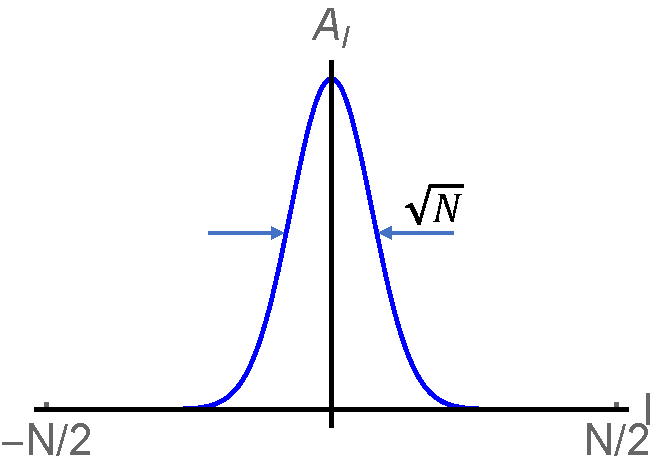
\includegraphics[height = 1in]{image/1-8-aGau.pdf}}
\subfigure[$U = + \infty$]
{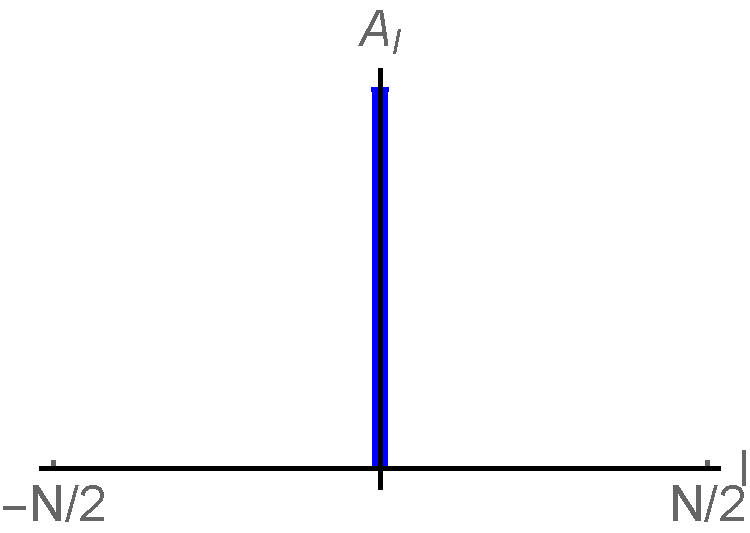
\includegraphics[height = 1in]{image/1-8-bDel.pdf}}
\caption{From non-interacting case to infinite repulsive interaction.}
\label{fig:1-8}
\end{figure}

Under repulsive interaction, it is called "Squeezed State", which the fluctuation is smaller than Gaussian distribution. This truth could be applied in accurate measurement.

Consider the general interaction. 
\begin{equation}
H_{int} \ket\psi  = U\frac{(n_1-n_2)^2}{4} \sum_l A_l \ket{l} = \sum_l U l^2 A_l \ket{l}
\end{equation}
\begin{equation}
a_1^\dag a_2 \ket l  = \sqrt{N/2+l+1}\sqrt{N/2-l} \ket{l+1} 
\end{equation}
In the limit $N \gg 1$, (the maximum of $|l|$ is $N/2$, $N/2+l$ is still in the order of $N$)
\begin{equation}
a_1^\dag a_2 \ket l = \sqrt{N^2/4-l^2}\ket{l+1}
\end{equation}
Thus
\begin{equation}
E A_l = -t \sqrt{N^2/4-l^2}(A_{l+1}+A_{l-1}) + Ul^2 A_l
\end{equation}
It has the same form of the system in the harmonic trap with non-uniform hopping. 
Transform the equation to the continuous form
\begin{equation}
E A_l = -t \frac{N}{2} \partial_l^2 A_l + (U l^2+ tl^2/N) A_l
\end{equation}

Assume the solution is in the following form
\begin{equation}
A_l = \frac{e^{-l^2/\sigma}}{(\pi \sigma /2)^{1/4}}
\end{equation}
Then, substitute this ansartz to the equation
\begin{equation}
\sigma = \sqrt{\frac{4}{N^2}+\frac{2U}{Nt}}
\end{equation}
Under the two limit $U = 0$ and $U = +\infty$, $\sigma(U)$ goes back to the case we discuss above.

Thus, we could see $\sigma(U) < \sigma(U = 0)$, i.e. the state is squeezed. It leads to a smaller fluctuation and increase the measurement precision.

\subsection{Attractive interaction}
The equation about $A_l$ is still valid under attractive interaction. However, it is no longer in a "Harmonic" trap, but an "anti-Harmonic" trap, $V_l =Ul^2$.
As a result, the "potential" makes the $A_l$ prefer to sit at largest $|l|$.

The infinite attractive interaction, $U = -\infty$ gives us a cat state.
\begin{equation}
\ket{GS, U=-\infty} = \frac{1}{\sqrt{2}\sqrt{N!}}\left(a_1^{\dag N}+a_2^{\dag N}\right)\ket{vac}
\end{equation}

Cat state is hard to realize in the experiments.
If we only focus on mathematics, we could easily have negative interaction among Bosons, and we could make the hopping $t$ extremely small. As as result we could achieve the case $U\rightarrow -\infty$ pretty easy. 
However, it is hard to have Bosons in Cat state. Currently, it is pretty hard to achieve the Cat state with hundreds of particles. It means, when we increase the number of particle, the Cat state dies. Why?
It goes back to the fact that the Cat state has huge fluctuation. Before, we calculated that $\Delta N /N \approx 1$. It means that the state is extremely
easy to be destroyed. And it is hard to keep the properties of Cat state during measurement.

In order to probe a cat state, we need a measurement reflecting $N$-particle operator. 
For example, a mixed state
\begin{equation}
\rho_{mix} = \frac{1}{2} (\ket{N,0}\bra{N,0} + \ket{0,N}\bra{0,N}) 
\end{equation}
can not be distinguished from the Cat state if we consider an $n$-particle operator, if $n<N$. More concretely, 
\begin{equation}
\braket{cat|\mathscr O^{(n)}|cat} = Tr (\rho_{mix} \mathscr O^{(n)})
\end{equation}
is valid for all $n$-particle operator $\mathscr O^{(n)}$, when $n<N$
In order to distinguish a Cat state, in principle, we need a $\infty$-particle operator. 
A simple idea is to consider time-evolution operator, $U = e^{i H t}$. The exponential in the time-evolution operator gives a $\infty$-particle operator.
\begin{equation}
e^{i H t} = \sum_{n=0}^\infty \frac{(iHt)^n}{n!}
\end{equation}
\section{Emergency of Coherence through measurement process}
Consider a $2N$-particle Fock State.
\begin{equation}
\ket{0} = \frac{1}{N!}a_1^{\dag N} a_2^{\dag N} \ket{vac}
\end{equation}
Here $a_i^\dag$, ($i= 1,2$) are creation operator of a photon with phase $\theta_i$.
The single particle density matrix is given by
\begin{equation}
\rho_{0} = N \left(\begin{array}{cc}
1 & 0\\
0 & 1
\end{array}\right)
\end{equation}
Considering a measurement process $c^\dag (\alpha a_1 + \beta a_2)$.
Experimentally, we could treat the process as two laser transiting a laser splitter.
In the following, let's simplify the process as $\alpha = \beta$.
Thus, the measurement process could be represented by acting the operator $(a_1+a_2)/\sqrt{2}$ on the state succesively.
\subsubsection{acting once}
\begin{equation}
\ket 1 =\frac{1}{\sqrt{2} } (a_1+ a_2)\ket{0} = \frac{\ket{N_1,N}+\ket{N,N-1}}{\sqrt{2}}
\end{equation}
The density matrix
\begin{equation}
\rho_1=N\left( \begin{array}{cc}
1 & 1/2\\
1/2 & 1
\end{array} \right)
\end{equation}
Thus we could see it starting to get off-diagonal elements, i.e. ODLRO.

\subsubsection{acting twice}
\begin{equation}
\ket 2 =  \frac{1}{\sqrt{2} }(a_1+ a_2)\ket{1} = \frac{1}{\sqrt{6}} \left(\ket{N-2, N} + 2\ket{N-1,N-1}+\ket{N,N-2}\right) 
\end{equation}
The density matrix
\begin{equation}
\rho_2 = N\left(\begin{array}{cc}
1 & 2/3\\
2/3 & 1
\end{array}\right)
\end{equation}
The OD elements become larger.

\subsubsection{Continue the measurement}
We could see, as the number of measurement increase, the coherence in the state increases as well.
We could image the process
\begin{equation}
h_1 = \lambda e^{-i\Omega t} c^\dag (a_1+a_2)+h.c.
\end{equation}
as a perturbed part in the Hamiltonian. And let the system involve. 
Then the operator $a_1 + a_2$ could act on the initial state infinite times.
And it could introduce the phase coherence in the system.


\end{document}
